\documentclass[11pt,a4paper]{article}

% --- Geometry & Margins ---
\usepackage[margin=20mm]{geometry}

% --- Typography & Font Setup ---
\usepackage{times}              % Times New Roman for entire document
\usepackage[T1]{fontenc}
\usepackage[utf8]{inputenc}
\usepackage{microtype}
\usepackage{setspace}
\setstretch{1.15}               % 1.15 line spacing

% --- Paragraph Formatting ---
\setlength{\parindent}{0pt}
\setlength{\parskip}{6pt}

% --- Packages for Tables & Layout ---
\usepackage{tabularx}
\usepackage{booktabs}
\usepackage{array}
\usepackage{subcaption}
\usepackage{graphicx}
\usepackage{float}
\usepackage{titlesec}
\usepackage{amsmath, amssymb}
\usepackage{fancyhdr}
\usepackage{xcolor}
\usepackage[colorlinks=true, linkcolor=blue, urlcolor=blue, citecolor=blue]{hyperref}

% --- Running Header & Footer ---
\pagestyle{fancy}
\fancyhf{}
\fancyhead[R]{\footnotesize\textcolor{gray}{CSE 4112: Machine Learning Laboratory \textbar\ Dataset Report}}
\fancyfoot[C]{\footnotesize\thepage}
\renewcommand{\headrulewidth}{0.4pt}

\begin{document}

\section*{EXPERIMENT: 13 Fruits ResNet-50 Layout}

\subsection*{1. Confusion Matrix (Single in a row, Bigger Form)}

\begin{figure}[H]
    \centering
    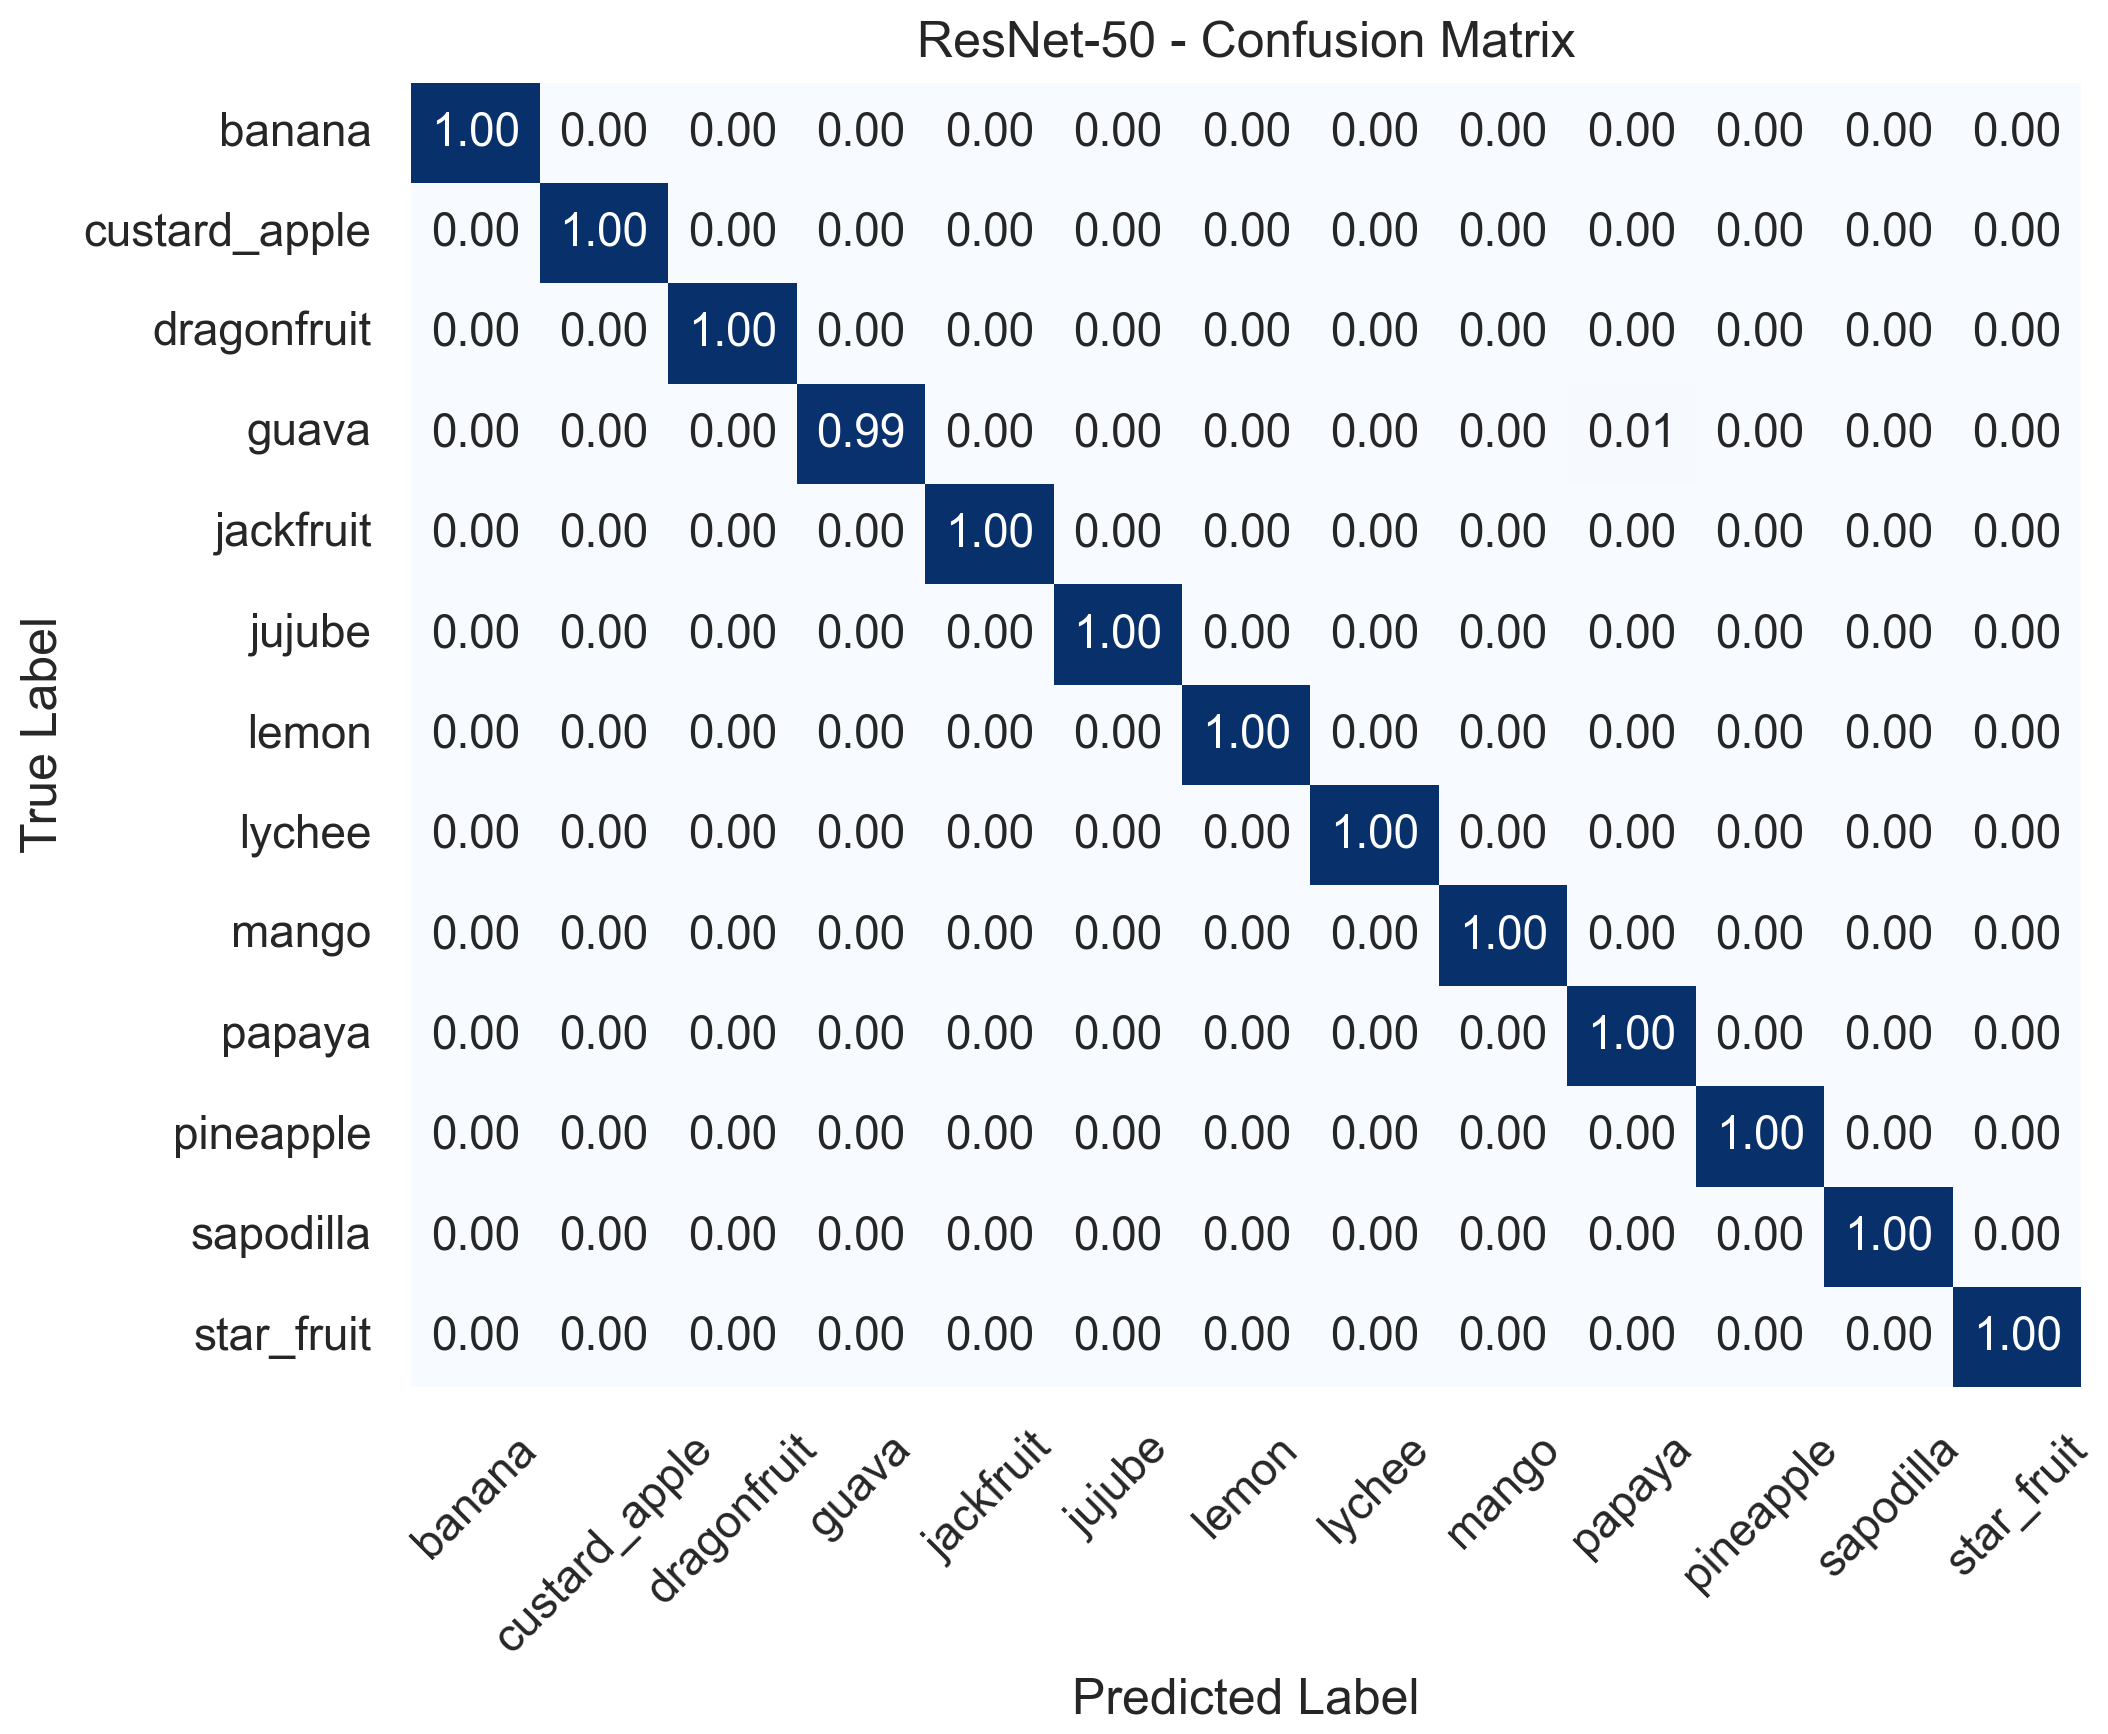
\includegraphics[width=0.75\textwidth]{figures/13_fruits_resnet50_confusion_matrix.png}
    \caption{All 13 Fruits: ResNet-50 (top model, 99.93\% accuracy) -- Normalized confusion matrix across 13 classes}
    \label{fig:exp-13fruits-cm}
\end{figure}

\subsection*{2. One-vs-Rest ROC Curves (Single in a row)}

\begin{figure}[H]
    \centering
    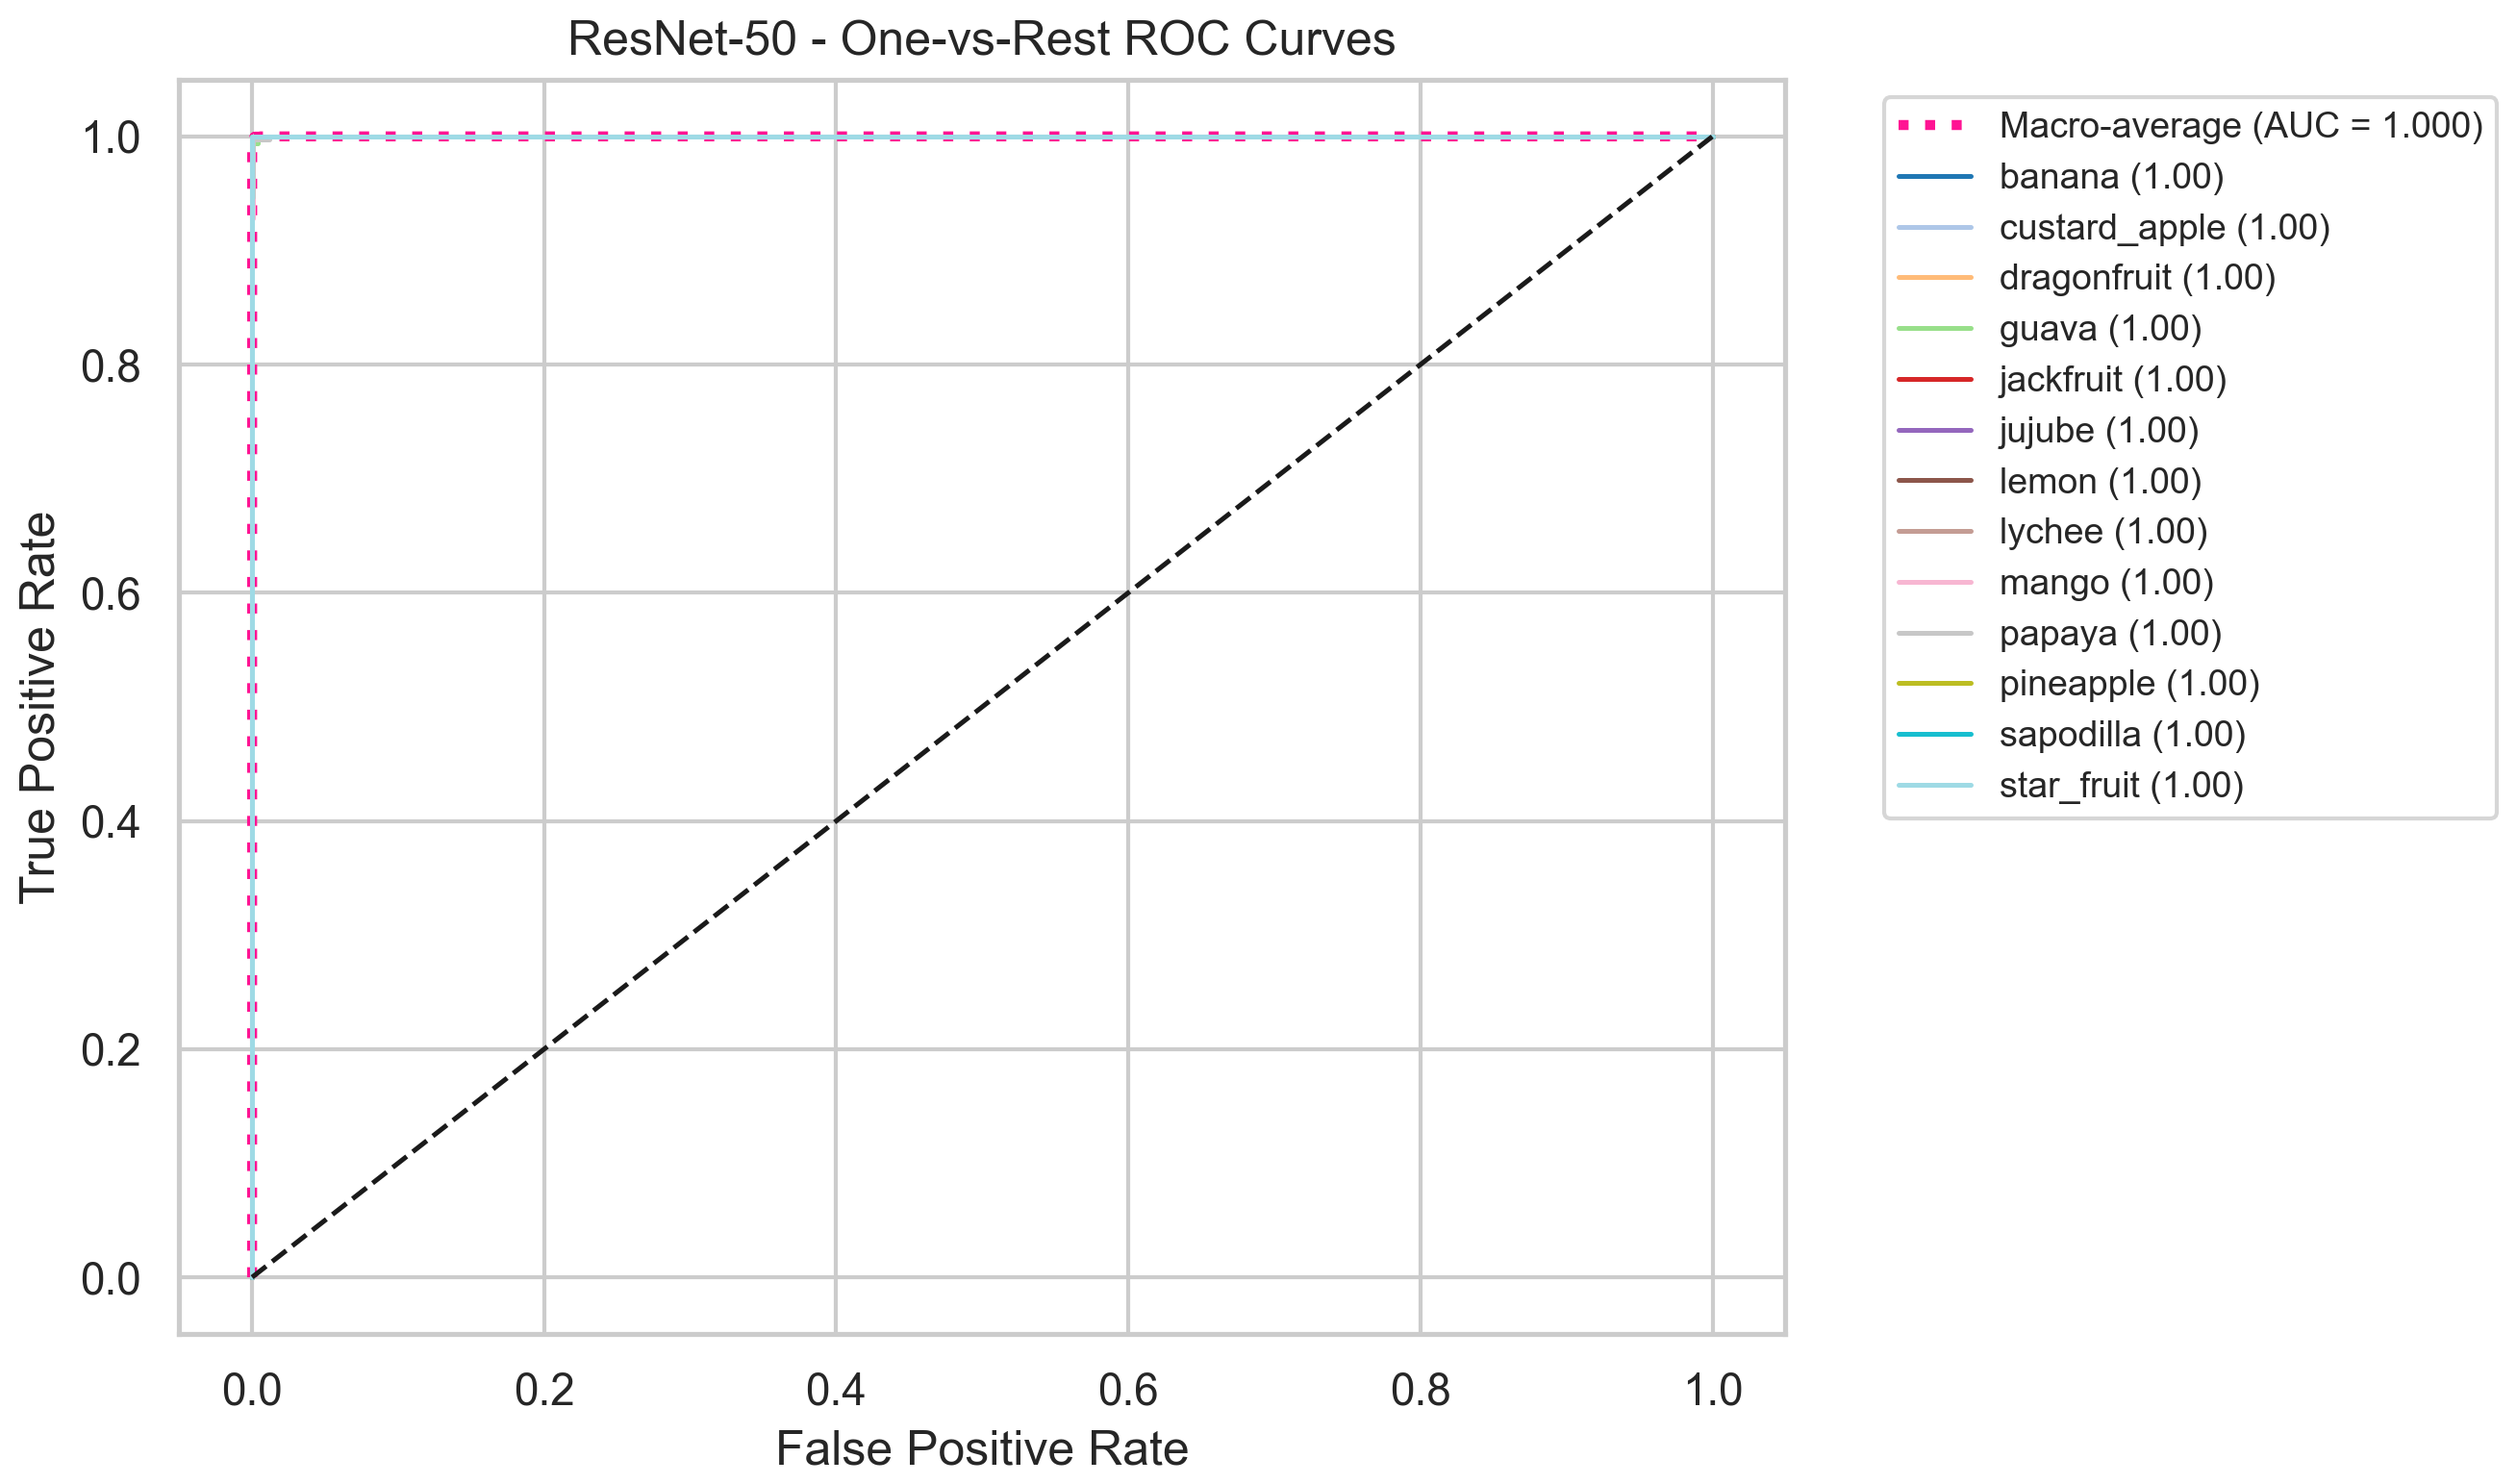
\includegraphics[width=0.75\textwidth]{figures/13_fruits_resnet50_roc_curves.png}
    \caption{All 13 Fruits: ResNet-50 -- One-vs-Rest ROC curves across all 13 fruit species (Macro-average AUC = 1.000)}
    \label{fig:exp-13fruits-roc}
\end{figure}

\newpage
\subsection*{3. Training \& Validation Curves (3 Plots in 2 Rows)}

\begin{figure}[H]
    \centering
    \begin{subfigure}[b]{0.48\textwidth}
        \centering
        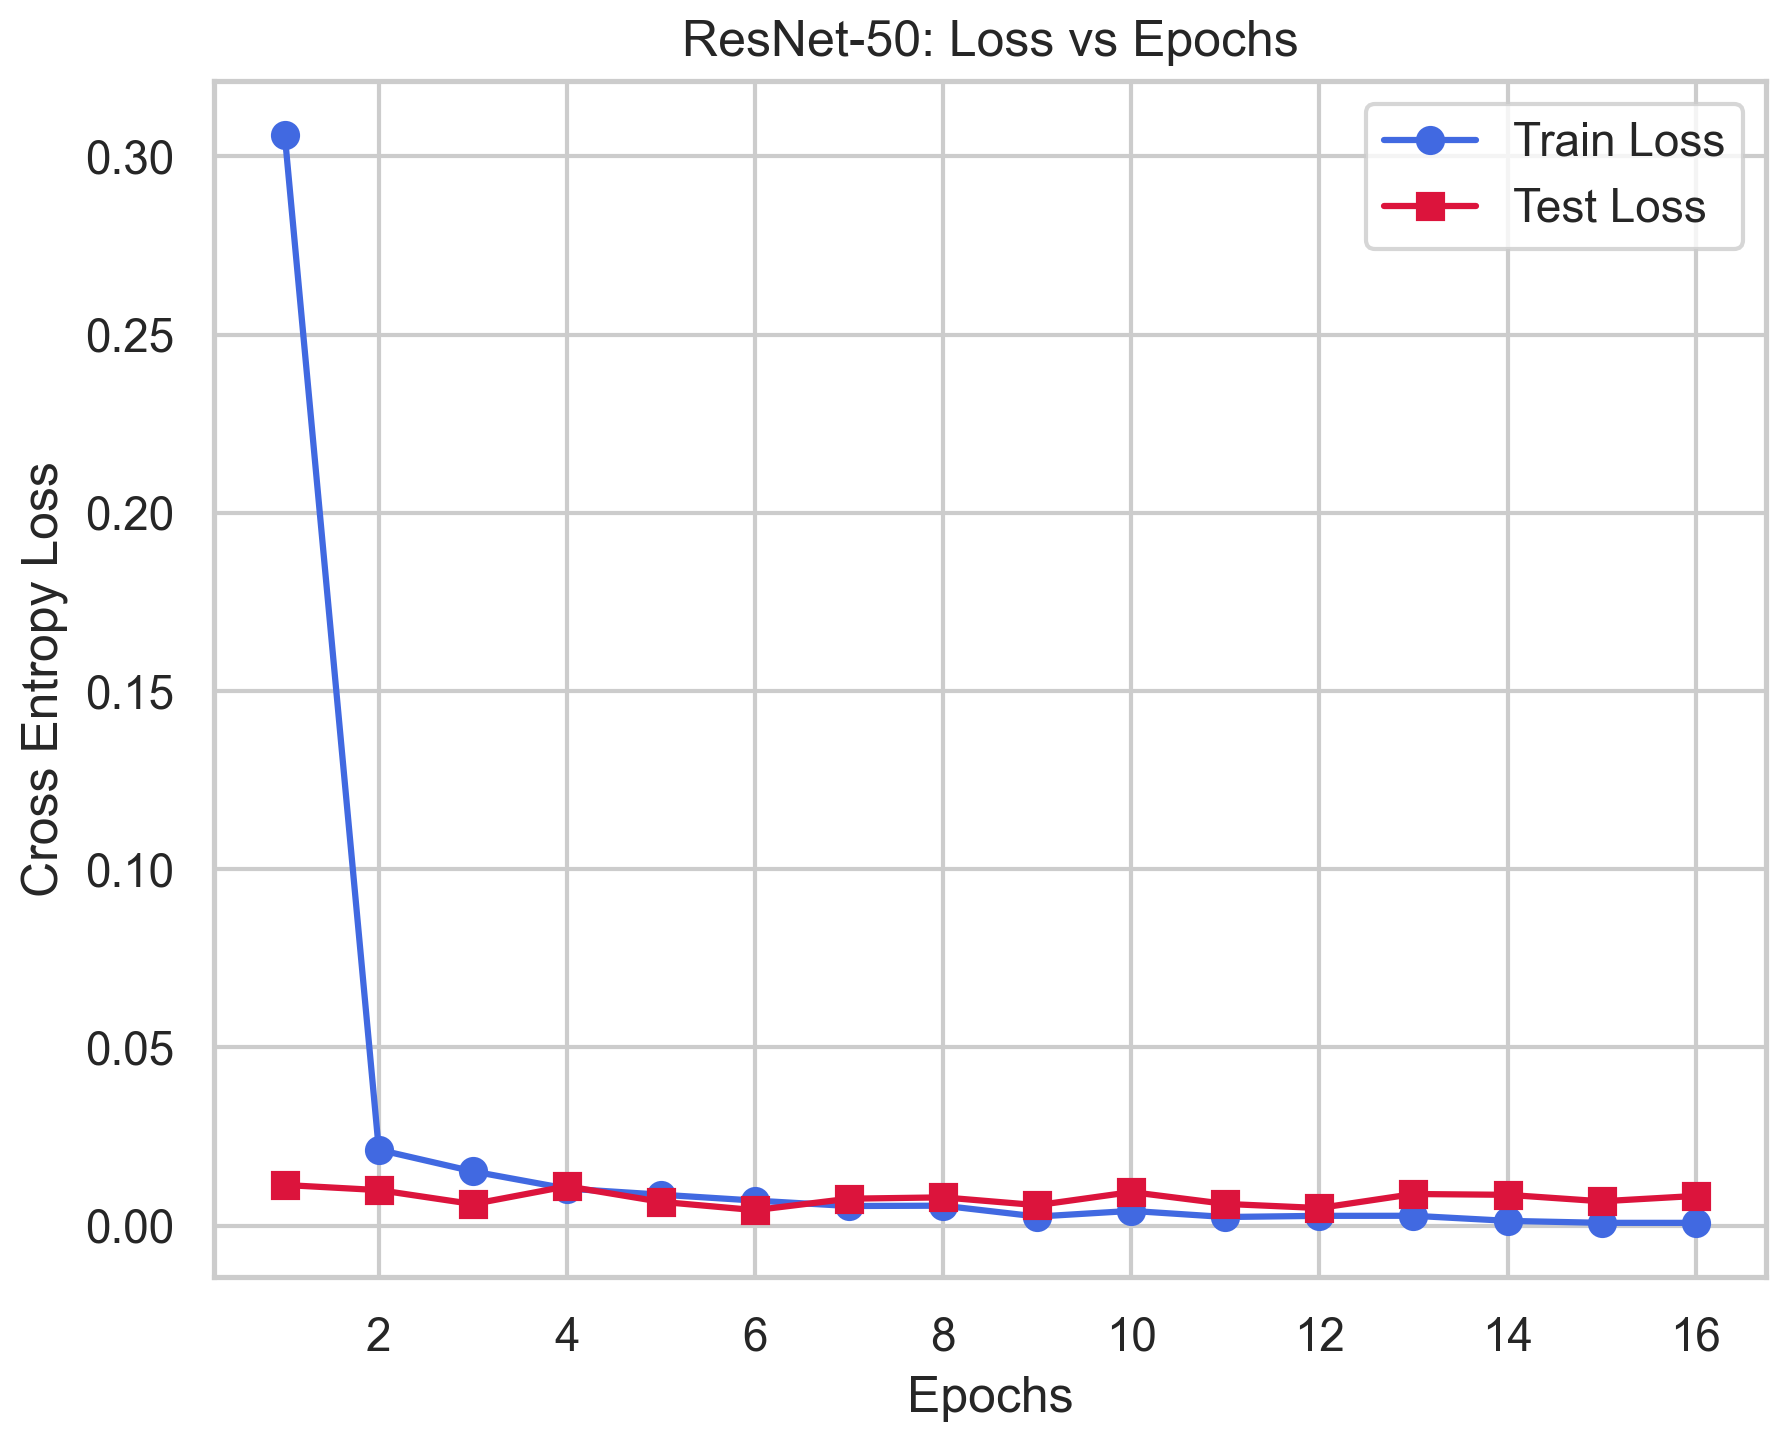
\includegraphics[width=\textwidth]{figures/13_fruits_resnet50_learning_loss.png}
        \caption{Loss vs Epochs}
        \label{fig:exp-lc-loss}
    \end{subfigure}
    \hfill
    \begin{subfigure}[b]{0.48\textwidth}
        \centering
        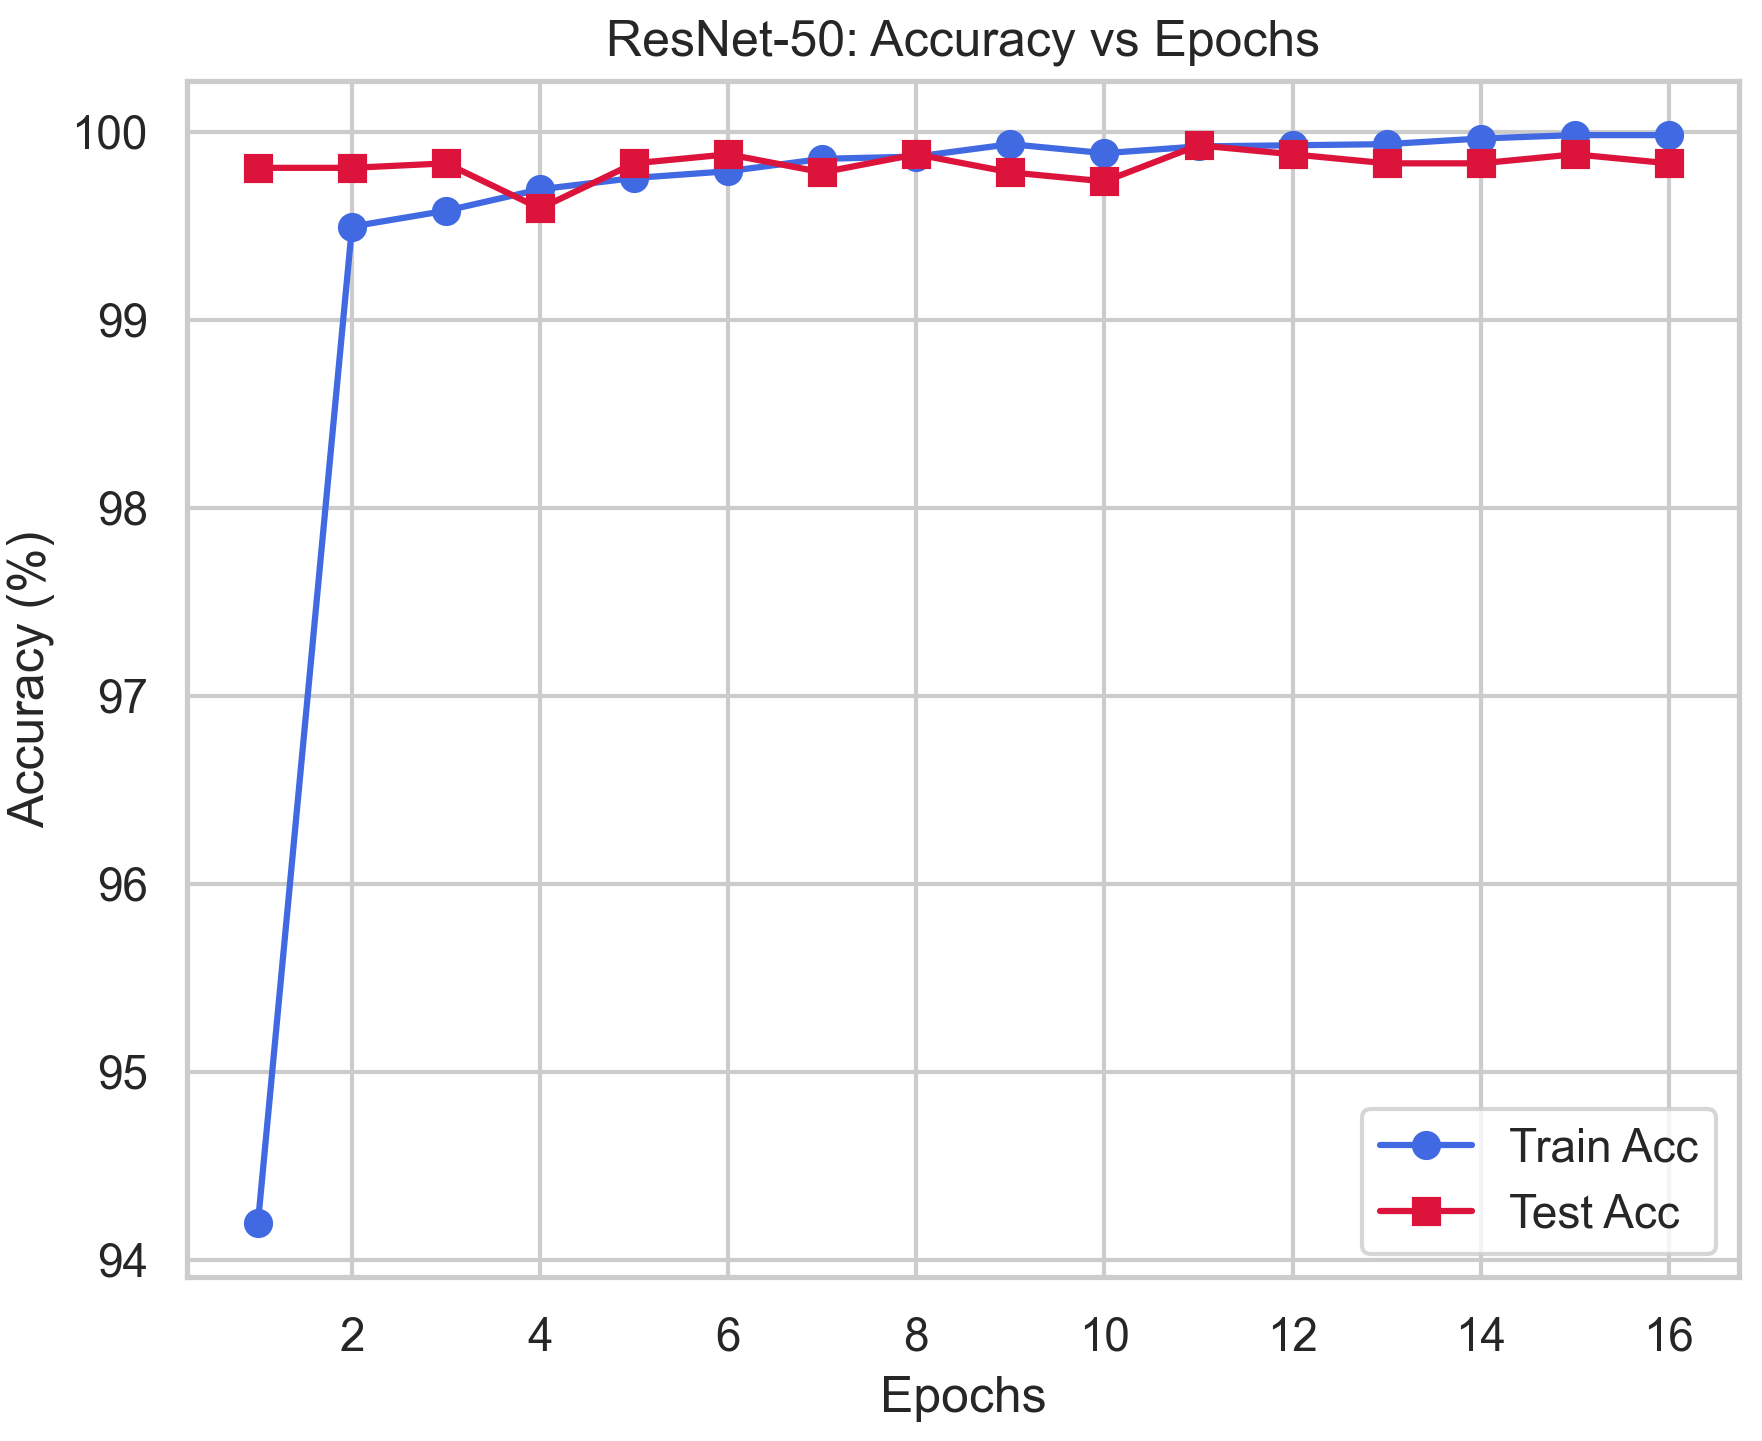
\includegraphics[width=\textwidth]{figures/13_fruits_resnet50_learning_accuracy.png}
        \caption{Accuracy vs Epochs}
        \label{fig:exp-lc-acc}
    \end{subfigure}
    \\[0.35cm]
    \begin{subfigure}[b]{0.48\textwidth}
        \centering
        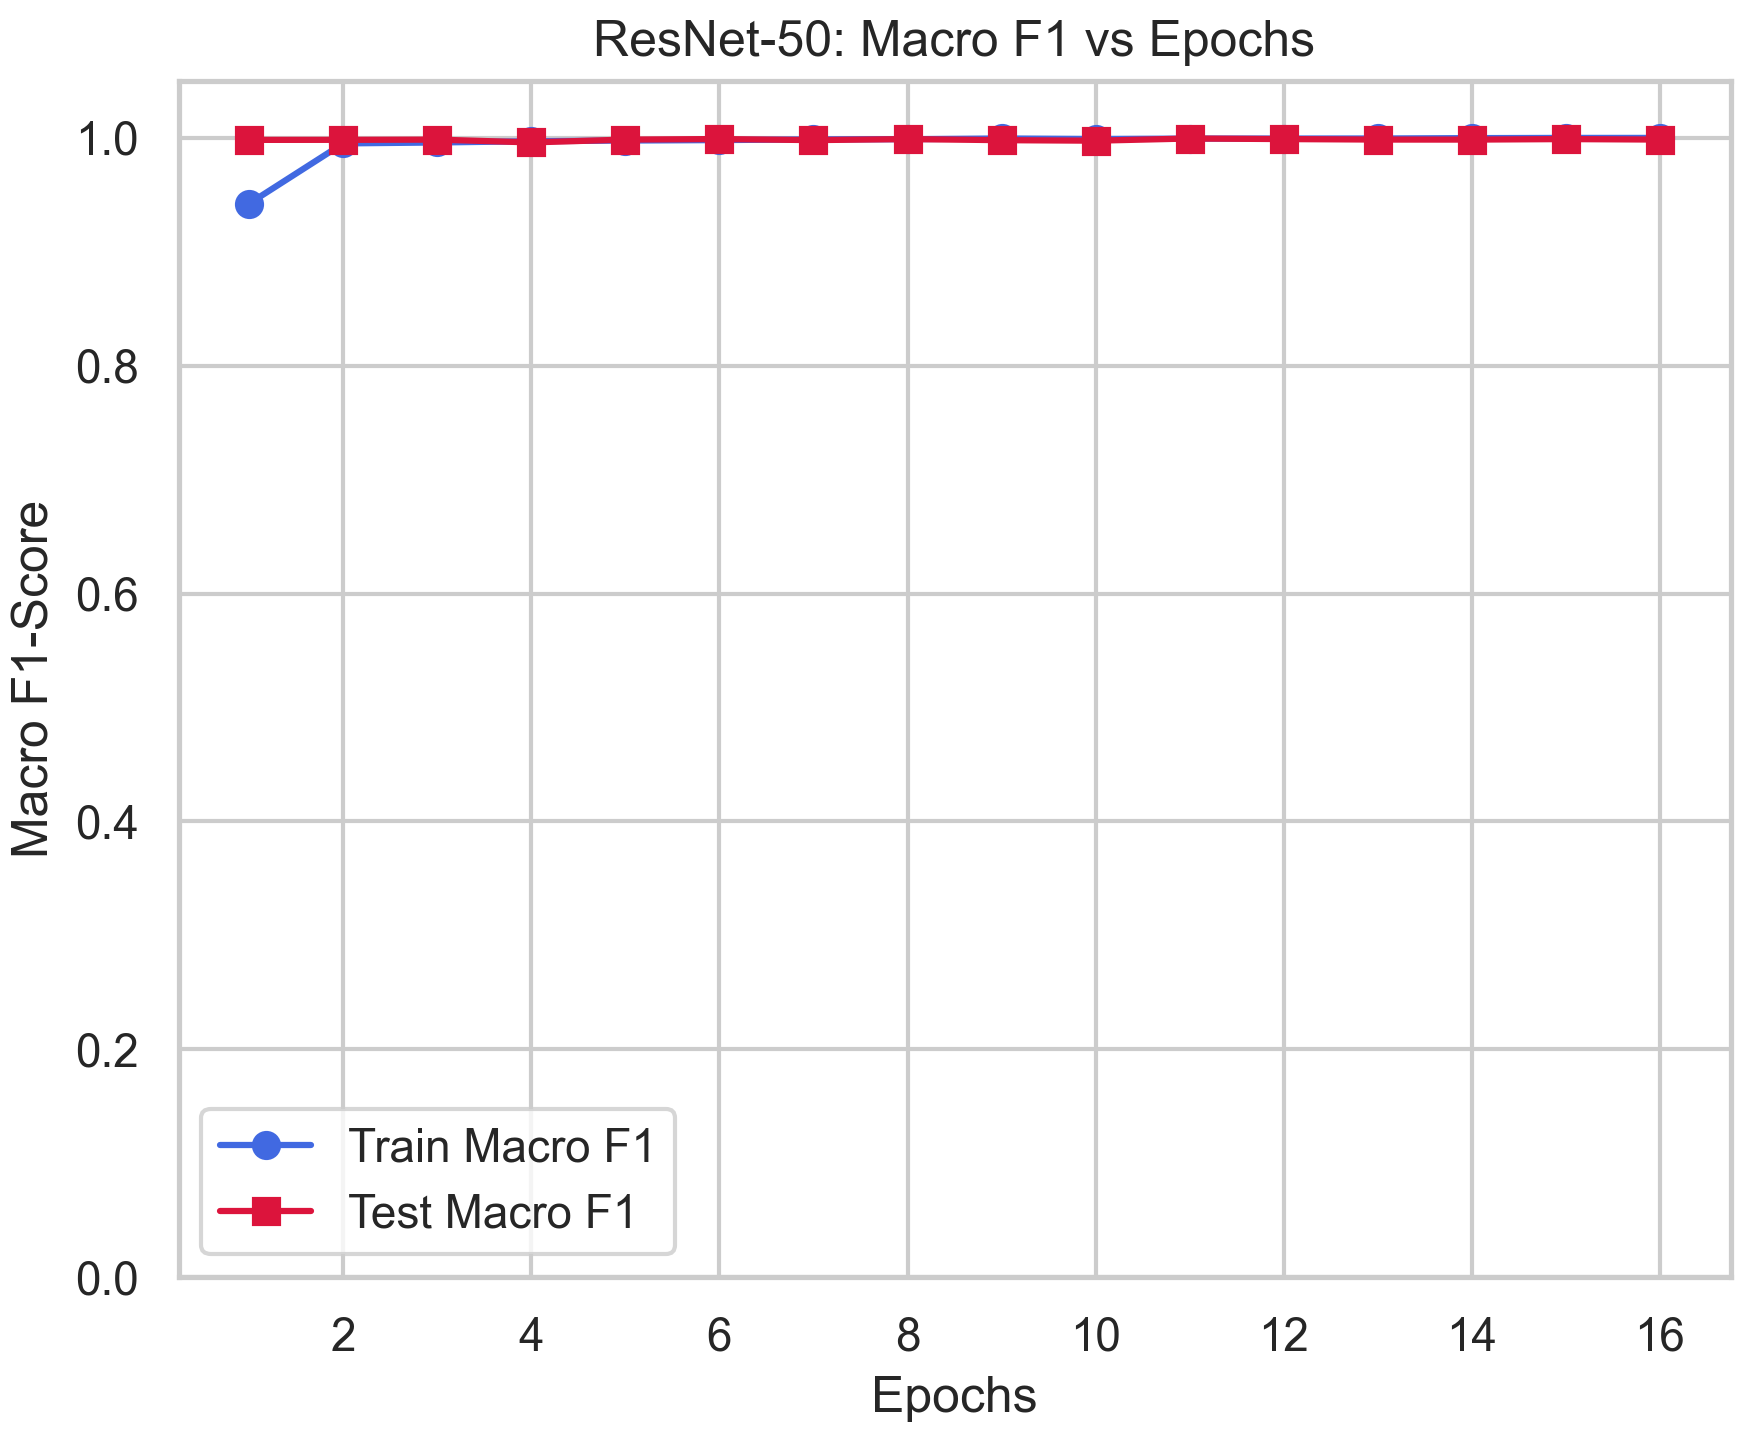
\includegraphics[width=\textwidth]{figures/13_fruits_resnet50_learning_macro_f1.png}
        \caption{Macro F1 vs Epochs}
        \label{fig:exp-lc-f1}
    \end{subfigure}
    \caption{All 13 Fruits: ResNet-50 -- Training and validation performance curves across epochs}
    \label{fig:exp-13fruits-lc}
\end{figure}

\end{document}
